\chapter{Analysis and Design} \label{chapter:4}
This chapter gives an overview of the overall system and explains the design choices made. Throughout the project, we explored various methods to implement a real-time augmented reality system for PWUs operating a wheelchair. Naturally, the structure and goals of the project have developed since the interim report, and we review the differences between the initial goals and final product .

\section{Design Overview}
As stated in the requirements, this project consists of three major components:
\begin{itemize}
	\item Human Detection and Direction (HDD)
	\item Object Mapping and Visualization
	\item Reactive Control on ARTA
\end{itemize}

\begin{figure}[ht]
	\centering
	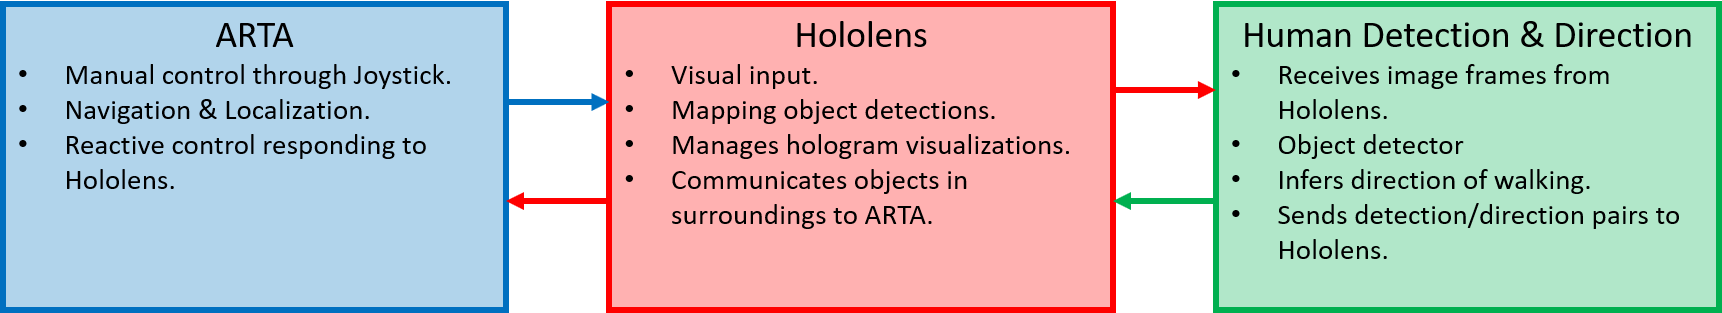
\includegraphics[width=1.0\linewidth]{img/chapter4_analysis/simpleSystemDiagram.png}
	\caption{High level system diagram showing the flow of messages from ARTA and the HDD system through the intermediary device, the Hololens.}
	\label{fig:simplifiedHL}
\end{figure}

From a very high level view, we can map these requirements to the respective devices they will be operating on. The HDD system takes implements the object detection and human direction inference, while the Hololens is responsible for utilizing the spatial mapping to obtain world positions of the detections, as well as visualizing the detections. The powered wheelchair (ARTA), has manual input that is overridden by the reactive control system that is dependent upon the detections and mappings. The diagram in Figure. \ref{fig:simplifiedHL} shows an overview of the system, and shows that the Hololens acts as an intermediary between ARTA and the HDD.

\subsection{Hardware}

\begin{table}[ht]
	\centering
	\begin{tabular}{l|l|l|l|}
		\cline{2-4}
		& \multicolumn{1}{c|}{\textbf{ARTA}}                                                 & \multicolumn{1}{c|}{\textbf{Hololens}} & \multicolumn{1}{c|}{\textbf{HDD}}                              \\ \hline
		\multicolumn{1}{|l|}{\textbf{Hardware}}         & \begin{tabular}[c]{@{}l@{}}Powered Wheelchair \\ controlled by Laptop\end{tabular} & Hololens                               & \begin{tabular}[c]{@{}l@{}}Desktop PC \\ with GPU\end{tabular} \\ \hline
		\multicolumn{1}{|l|}{\textbf{Operating System}} & Ubuntu 16.04                                                                       & UWP                                    & Ubuntu 16.04                                                   \\ \hline
	\end{tabular}
	\caption{Hardware description of devices each system runs on.}
	\label{tab:hardware}
\end{table}

Table. \ref{tab:hardware} summarises the hardware overall system is implemented on. The powered wheelchair, ARTA, is controlled by a laptop, which is responsible for the wheelchair speed, wheel rotations, navigation and localisation. The Hololens is a self contained augmented reality headset, running the Universal Windows Platform (UWP) operating system. Finally, the Human Detection \& Direction system is implemented on a desktop computer with a GTX 1050Ti GPU, allowing it to run real time object detectors.

\subsection{System Communication} \label{sec:systemComms}

\subsubsection{Robotic Operating System} Since the project spans multiple operating systems, we have chosen to utilize the Robotic Operating System (ROS) as a means of communication between the devices. In ROS, a \textit{node} is defined as a process that performs a computation. A node can be made up of smaller nodes that perform specific computations that serve the needs of the parent node. We can think of the three major systems as large ROS nodes that consists of smaller nodes that run individual tasks, such as creating the camera stream, or detecting objects.

\paragraph{ROS Topics} Nodes in ROS communicate with one another by publishing data in the form of \textit{messages} which get broadcasted over a \textit{topic}. Nodes can choose what data they receive by subscribing to topics. This method allows for nodes running on different devices to communicate with each other, regardless of the operating system. The nodes are unaware that the data it receives is published from a node running on a separate computer, making ROS a perfect choice for communication in this design.

\section{Human Detection \& Direction System}
The HDD system is responsible for detecting and predicting the directions of people in the surroundings of the wheelchair. By taking visual inputs in the form of images from the Hololens, we run an object detector trained on a dataset of pedestrians to detect people and heads. The bounding boxes produced by the object detector are fed as inputs to an object tracker and a body pose estimator. We use the results of these two nodes to infer the direction a detected person is moving in, and publish the results back to the Hololens.


We present an overall view of the HDD System, covering the purpose and design of individual components. We also propose the reasoning behind certain design choices, which we cover in more depth later in this report.

\subsection{YOLO Object Detector} \label{sec:yolo}
Object detectors often form the input to an object tracker or pose estimation system \cite{Bewley2016, Jin2017}. In the case of top-down body pose estimation methods, detections can be the first point of failure \cite{Insafutdinov}. As such, the accuracy of the chosen object detector must be considered, together with the choice of using a pre-trained model or training on a more relevant dataset. Finally, we must also consider the use-case of the detector, which must be able to operate in real-time and detect moving objects as they pass by.

\subsubsection{Choice of Detector}
As commented on in Section \ref{sec:detector}, modern deep learning techniques outperform classical object detectors in accuracy, but are limited by the requirement of a GPU to perform in real-time. Since the Hololens does not have built in support to run object detection networks, Microsoft provides the Azure Cognitive Services API to allow developers to query their system for object detections. The limitation is that this service is not free, and abstracts away the implementation of an object detector. Furthermore, one of the personal goals for this project was to learn more about CNNs in computer vision.

\paragraph{} Taking this into account, we compared several deep learning architectures for object detection. Previous work done in the PRL used Facebook AI Research's (FAIR) Detectron to detect objects \cite{Chacon-Quesada, Detectron2018, Rena}. Further discussions with members of the Imperial Computer Vision \& Learning Lab suggested the use of the YOLO object detector \cite{Redmon}, due to its speed and having a lightweight implementation that could be run on lower end GPUS at relatively high frame rates. This prompted the design decision to use the Darknet framework to use the \textbf{YOLOv3-tiny} architecture as the object detection method of choice for this project \cite{Redmon2018}.

\subsubsection{Pre-trained Model vs Training} \label{sec:designYOLO}
An advantage of using the YOLO Darknet framework is that it provides trained models which can detect multiple object classes, including the class \textit{Person}. One of the pre-trained models is the YOLOv3-tiny architecture trained on the Common Objects in Context (COCO) dataset \cite{Lin}.

\paragraph{Comparing Models} To compare the accuracy of the bounding boxes produced by pre-trained model, sample videos were recorded using the Hololens and used as a base comparison point. It was quickly shown that although the COCO trained model can detect individuals, or multiple people who are well spaced out, it had difficulty in differentiating between people who are close together or slightly occluded. Figure \ref{fig:yoloCHvsCoco} highlights the issue of the COCO model failing to detect small people close together.

\begin{figure}[ht]
	\begin{subfigure}[b]{.5\textwidth}
		\centering
		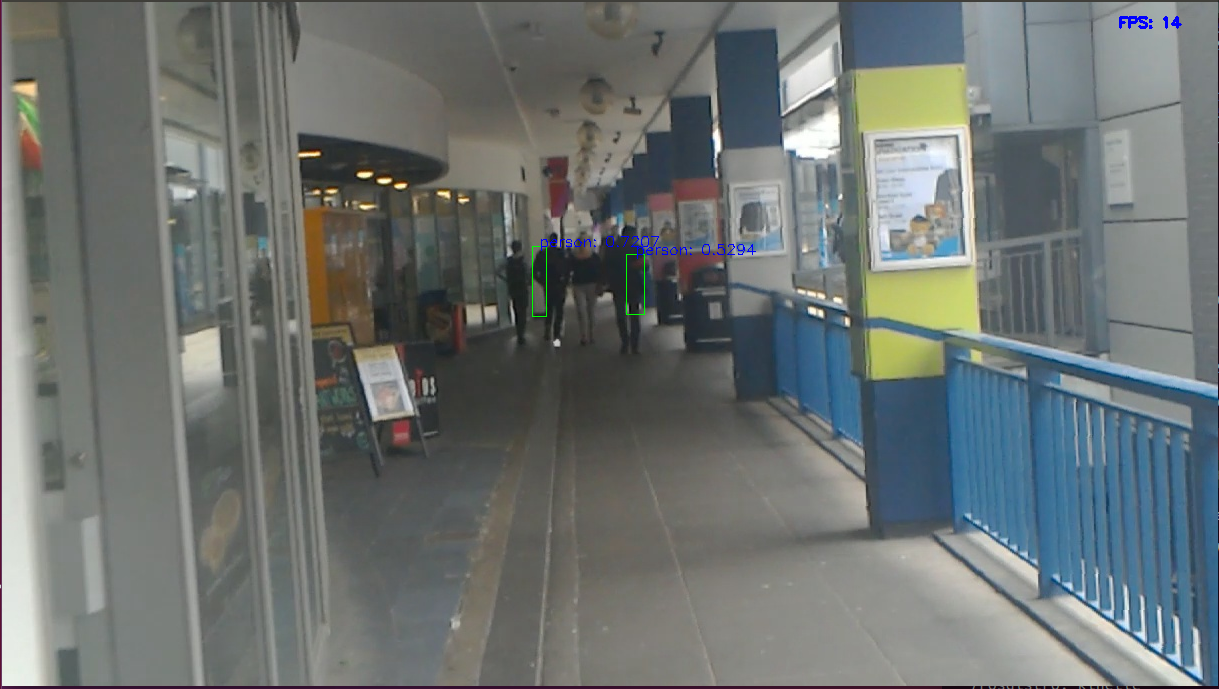
\includegraphics[width=0.95\linewidth]{img/chapter4_analysis/yoloCoco.png}
		\caption{COCO YOLOv3-tiny}
	\end{subfigure}%
	\hspace{\fill} 
	\begin{subfigure}[b]{.5\textwidth}
		\centering
		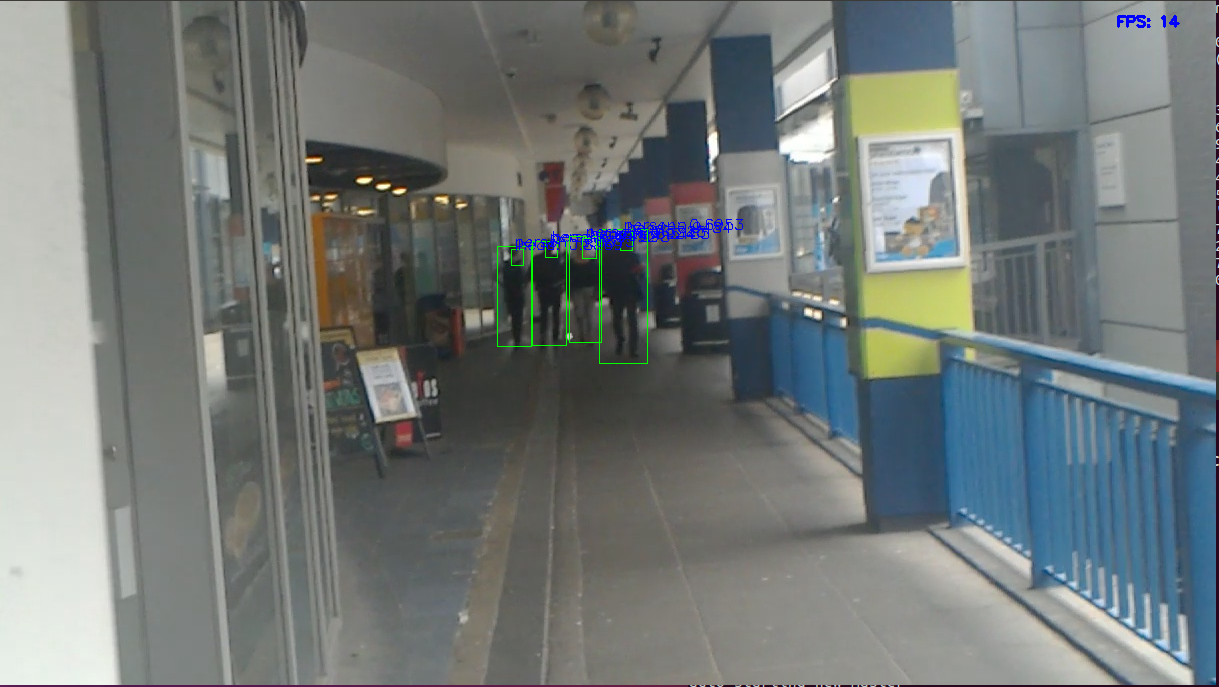
\includegraphics[width=0.95\linewidth]{img/chapter4_analysis/yoloCH.png}
		\caption{Trained YOLOv3-tiny}
	\end{subfigure}
	\vspace{-2\baselineskip}
	\begin{center}
		\caption{Model comparison on a video from Sherfield Walkway at Imperial College London. The trained model is able to better detect figures at a distance.}
		\label{fig:yoloCHvsCoco}
	\end{center}
	\vspace{-2\baselineskip}
\end{figure}

\paragraph{Pedestrian Dataset} A common case in pedestrian detection is occlusion, where only certain parts of an individual are visible.  To resolve this issue, we decided to train the YOLOv3-tiny model on the \textbf{CrowdHuman} dataset \cite{Shao}, which contains annotated images of people in crowded places. The annotations include bounding boxes for the head, visible human region and full-body region. The annotations for partially visible people allows the network to learn to recognize occlusions, reducing the issue of failed detections when people are too close to each other. We also trained the network to detect heads, since we initially wanted to use head pose estimation to determine direction.

\paragraph{Analysis}
The result of training the YOLOv3-tiny model on the CrowdHuman dataset is that the system is able to better detect smaller figures with obscured bodyparts. The additional ability to detect heads allowed us to explore the use of head pose estimation for direction inference. We go into further detail on the training process in the Implementation section of this report.

\subsection{YACHT: Yet Another Crowd Human Tracker}
The bounding boxes produced by the object detector are consumed by the \textbf{Yet Another Crowd Human Tracker} (YACHT) module, which is made up of two nodes. The tracker node uses the Deep SORT algorithm to track detected individuals \cite{Wojke2018}, while the pose estimator node uses the OpenPose \cite{Cao2017} network to determine whether a person is walking towards or away from the PWU.

\paragraph{}In the following sections, we briefly explain the  methods used to infer the directions people are walking in. We also explore the use of head pose estimation, and the limitations that prevented it from making it to the final design.

\subsubsection{YACHT Tracker: Object Tracking} \label{sec:YACHT}
We explored existing object tracking methods in Section \ref{sec:objectTrack} and discussed our choices in \ref{sec:objectTrackComments}. For moving object tracking on a powered wheelchair, we express the need for an online object tracking system. As such, we chose to investigate two related real-time methods, SORT \cite{Bewley2016} and Deep SORT \cite{Wojke2018}.

\paragraph{SORT}  The Simple Online and Real-time Tracking (SORT) method is a fast online object tracker. The initial implementation of YACHT used the SORT algorithm due to its speed. However, it was quickly realized that due to the simplicity of the association metric, object tracking was not very accurate, especially for occluded objects. When two objects crossed paths, the tracker was unable to recognize the act, and re-labelled the objects with brand new tracking IDs.

\paragraph{Deep SORT} Deep SORT is an extension of the original SORT algorithm, but uses a deep network to generate feature descriptors for the predicted bounding boxes. We explain the algorithm in Section \ref{sec:objectTrack}, but to repeat, instead of using the Intersection-over-Union association metric to compare bounding boxes, the deep network generates feature descriptors for the bounding box, and a Nearest-Neighbours is used to compare the features with a library of feature vectors for each tracked object. This is a form of person re-identification, and this additional step reduced the problem of trackers being lost due to occlusion.

\begin{figure}[ht]
	\centering
	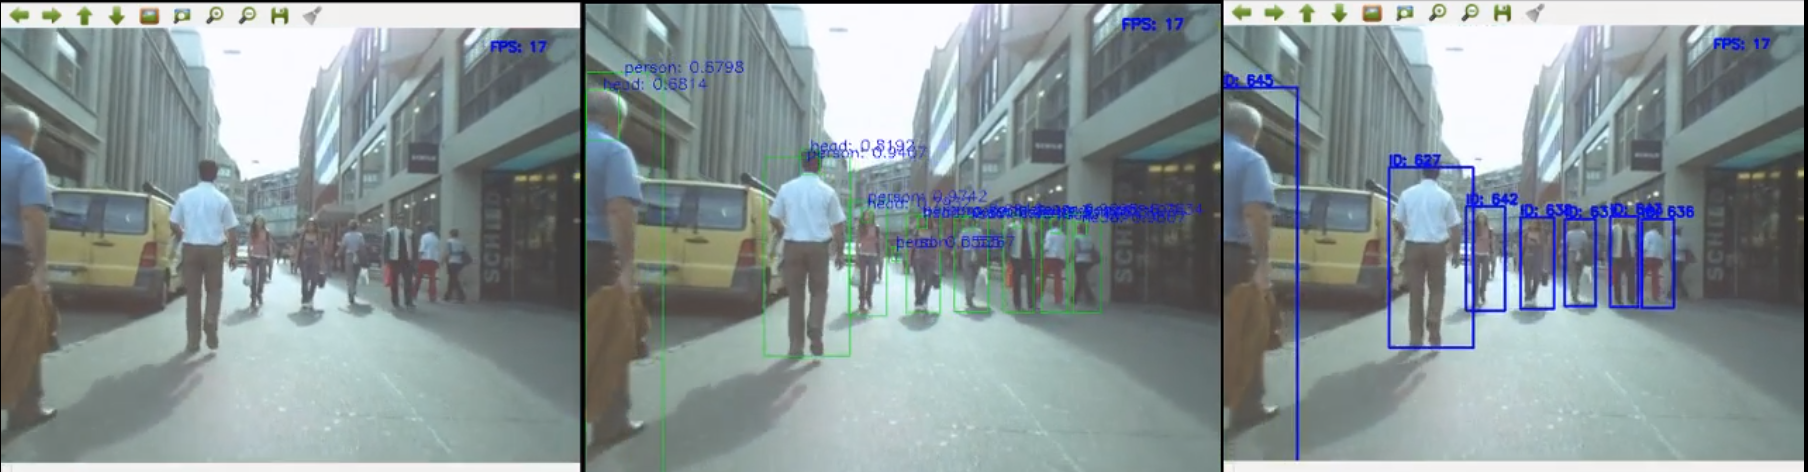
\includegraphics[width=1.0\linewidth]{img/chapter4_analysis/deepSortMOT.png}
	\caption{MOT16 benchmark \cite{Milan} (L) using our YOLO model (M) for Deep SORT (R). The increased detection accuracy results in slightly better initial detections, so tracking is more accurate.}
	\label{fig:deepSortMOT}
	\vspace{-1\baselineskip}
\end{figure}

\paragraph{Analysis} The generation and storage of feature descriptors for tracks is an expensive process. For the system to run in real-time, a GPU is needed to accelerate the network. We have made changes to the Deep SORT implementation so it can run on Tensorflow-GPU, which we explain later in this report. This improves the speed significantly, but uses up precious memory. As a result, we had to consider the amount of memory available on the GPU, since the YOLO detector and OpenPose networks also rely on GPU acceleration. After testing, we found that it was possible to run both networks on the GPU at the same time, and we chose to use the Deep Sort method.

\newpage
\subsubsection{Object Tracking for Direction Inference} \label{sec:objecTrackingDirection}
An idea we explored was to use the previous image co-ordinates of a tracker to predict the direction a person will walk in. This involved storing the previous states of each track and extrapolating the centroids of each track to determine a direction.

\begin{figure}[ht]
	\begin{subfigure}[b]{.45\textwidth}
		\centering
		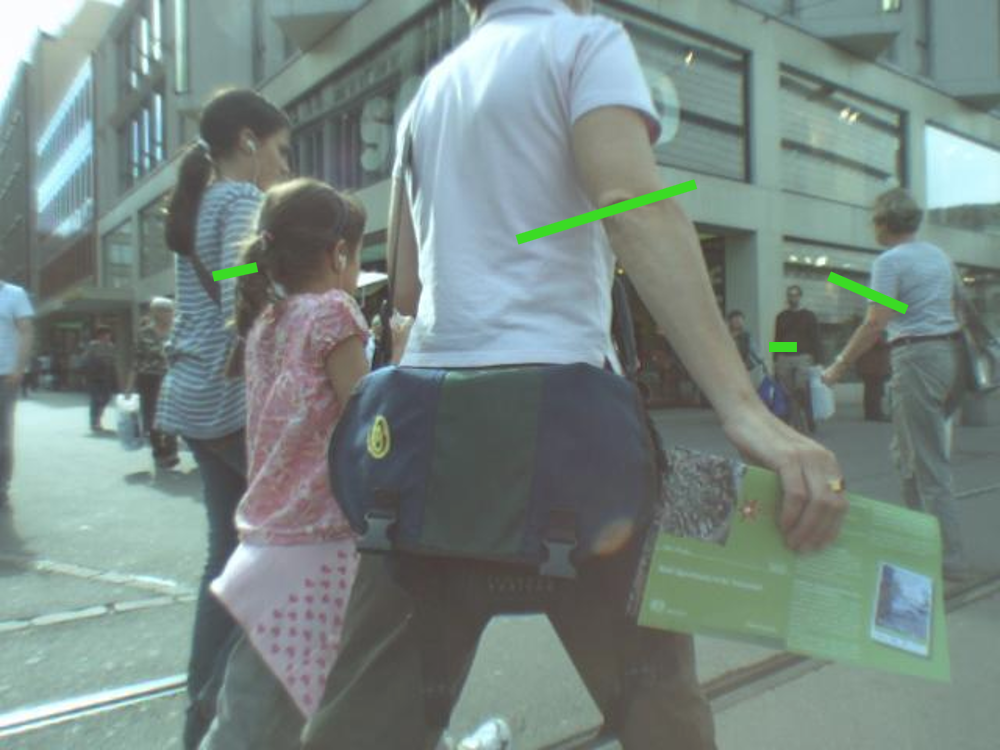
\includegraphics[width=1.0\linewidth]{img/chapter4_analysis/linExDirection.png}
		\caption{Tracks with horizontal motion}
	\end{subfigure}%
	\hspace{\fill} 
	\begin{subfigure}[b]{.45\textwidth}
		\centering
		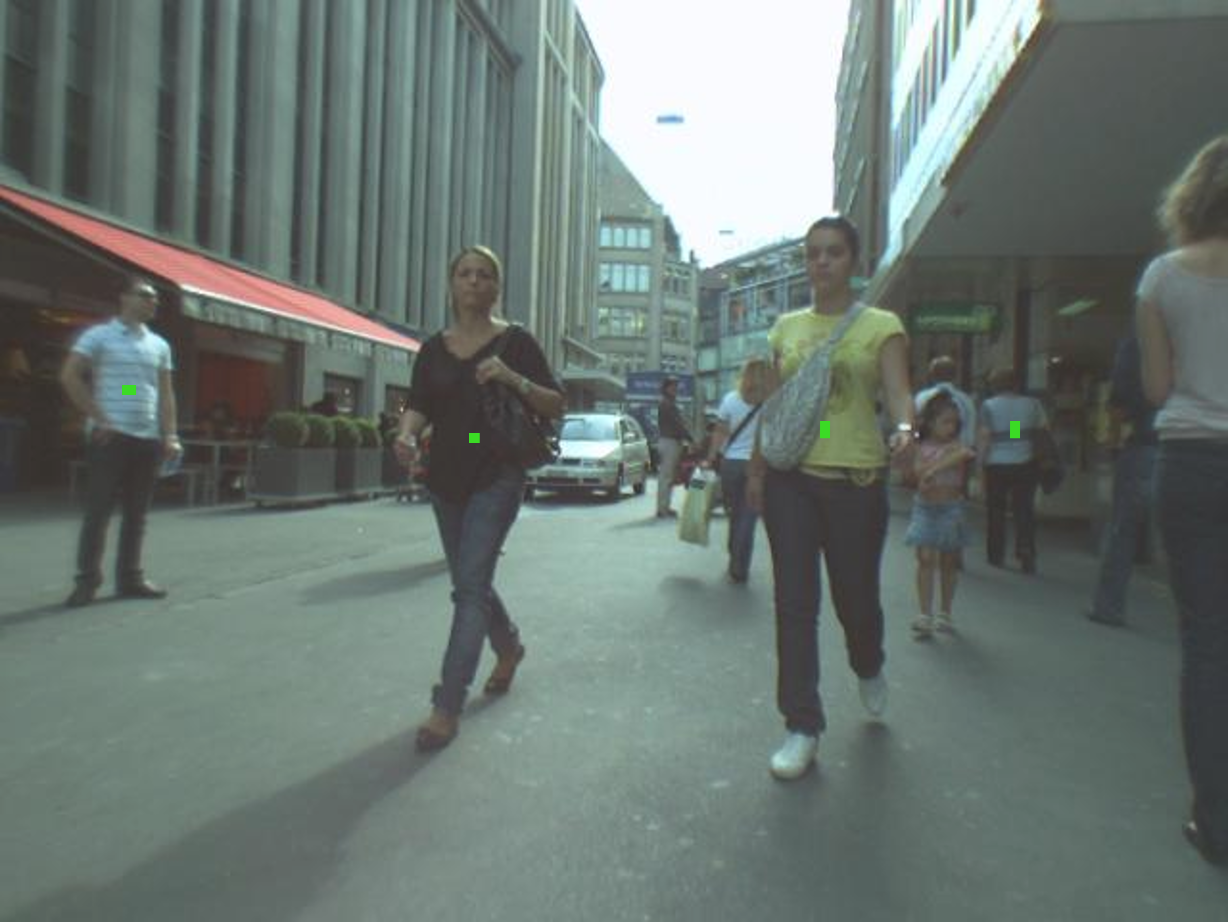
\includegraphics[width=1.0\linewidth]{img/chapter4_analysis/linExDirectionAmb.png}
		\caption{Tracks with mostly vertical motion}
	\end{subfigure}
	\vspace{-1\baselineskip}
	\begin{center}
		\caption{Linear extrapolation works for objects that move across the frame, but it becomes difficult to determine the direction when mostly vertical motion occurs}
		\label{fig:linExProblem}
	\end{center}
	\vspace{-2\baselineskip}
\end{figure}

\paragraph{Algorithm} For each tracked object in a frame:

\begin{algorithm}[ht] 
	\KwData{(x,y) centroid image co-ordinates up to the previous 5 states}
	\KwResult{(x,y) of extrapolated point}
	
	\For{Frame}
	{
		\For{Tracker}
		{
			\If{Tracker existed in previous frame}
			{
				Extrapolate over the centroids of previous states; \\
				Return linear extrapolation (x,y);
			}
			\If{Tracker has no previous states}
			{
				Add (x,y) centroid of tracker to queue of previous states;	\\
				Return current centroid (x,y);
			}
		}
	
	}
\end{algorithm}

\paragraph{Issues} Although the method works for trackers which cover large distances across the frame, linear extrapolation of image co-ordinates suffers when the tracked centroid does not have much horizontal motion. As such, this leads to an ambiguous definition of the direction. Since the object is not moving across the screen, it is not possible to differentiate between a person standing still, moving directly towards the PWU or walking away.

\begin{figure}[ht]
	\centering
	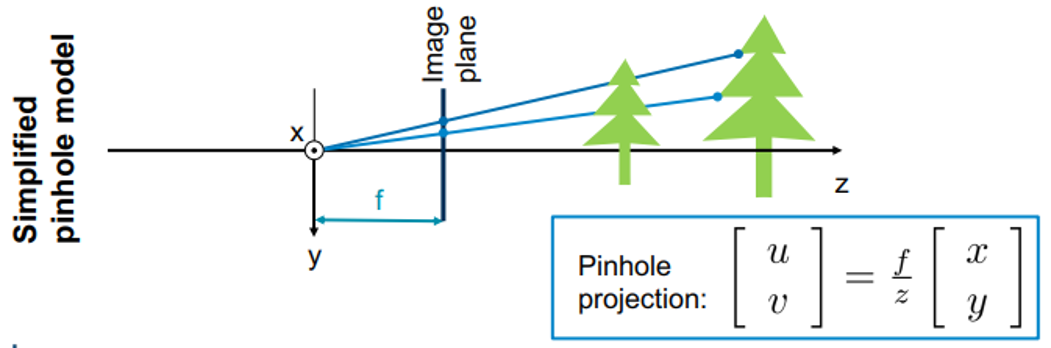
\includegraphics[width=0.8\linewidth]{img/chapter4_analysis/pinholecamera.png}
	\caption{Pinhole Camera projection and the loss of the z-axis \cite{Leutenegger2019}. As such, it is not possible to determine the exact distance to an object without a depth camera.}
	\label{fig:pinhole}
	\vspace{-1\baselineskip}
\end{figure}

\paragraph{} In the pinhole camera model, when an object in the real world is projected onto a 2D image, we lose the distance along the z-axis. The issue of a world-to-camera image projection occurs when we want to obtain the world co-ordinate of an object from the image. Due to the loss of z-axis information, the best we can do is to calculate a ray through the 2D image point. However, as shown in Figure \ref{fig:pinhole}, it becomes impossible to tell how far away the object is without a depth camera, since the object can exist anywhere along that ray.

\subsubsection{YACHT Direction: Body Pose Estimation} \label{des:YACHTBody}
To solve the direction ambiguity brought up in Section \ref{sec:objecTrackingDirection}, we proposed the use of body pose estimation techniques to determine whether a person is walking towards or away from the camera of the PWU. We researched several body pose implementations in Section \ref{sec:backBodyPoseEstimation}, but we ultimately decided on OpenPose, due to its well documented implementation on GitHub \cite{Cao2017}.

\paragraph{Object Detectors \& Bottom-Up Approaches} The YOLO object detector outputs the original image and the associated bounding box co-ordinates of detections. The OpenPose node consumes the image and performs body pose estimation on the whole image, before matching poses with the object detections. Since OpenPose is a bottom-up approach, we admit that it is counter-intuitive to use an object detector to detect individual people when OpenPose determines the body part key-points across the whole image. This will be explored more in the evaluation of the report.

\paragraph{Keypoint Estimation} \label{des:body_25}
The OpenPose framework provides several pre-trained models for body pose keypoint estimation. From our tests, we found that the \textit{BODY\_25} model was the fastest, suiting our real-time requirements. Figure \ref{fig:bodyKeyPoints} shows the key-points generated by the model. The model identifies 25 key-points on the human body, and can differentiate between the left and right limbs on the human body. This makes the model suitable for determining if a person is facing the camera or not. We further explain the methodology in the implementation section of the report. From this, the node outputs the direction of the object to the Hololens.

\begin{figure}[ht]
	\centering
	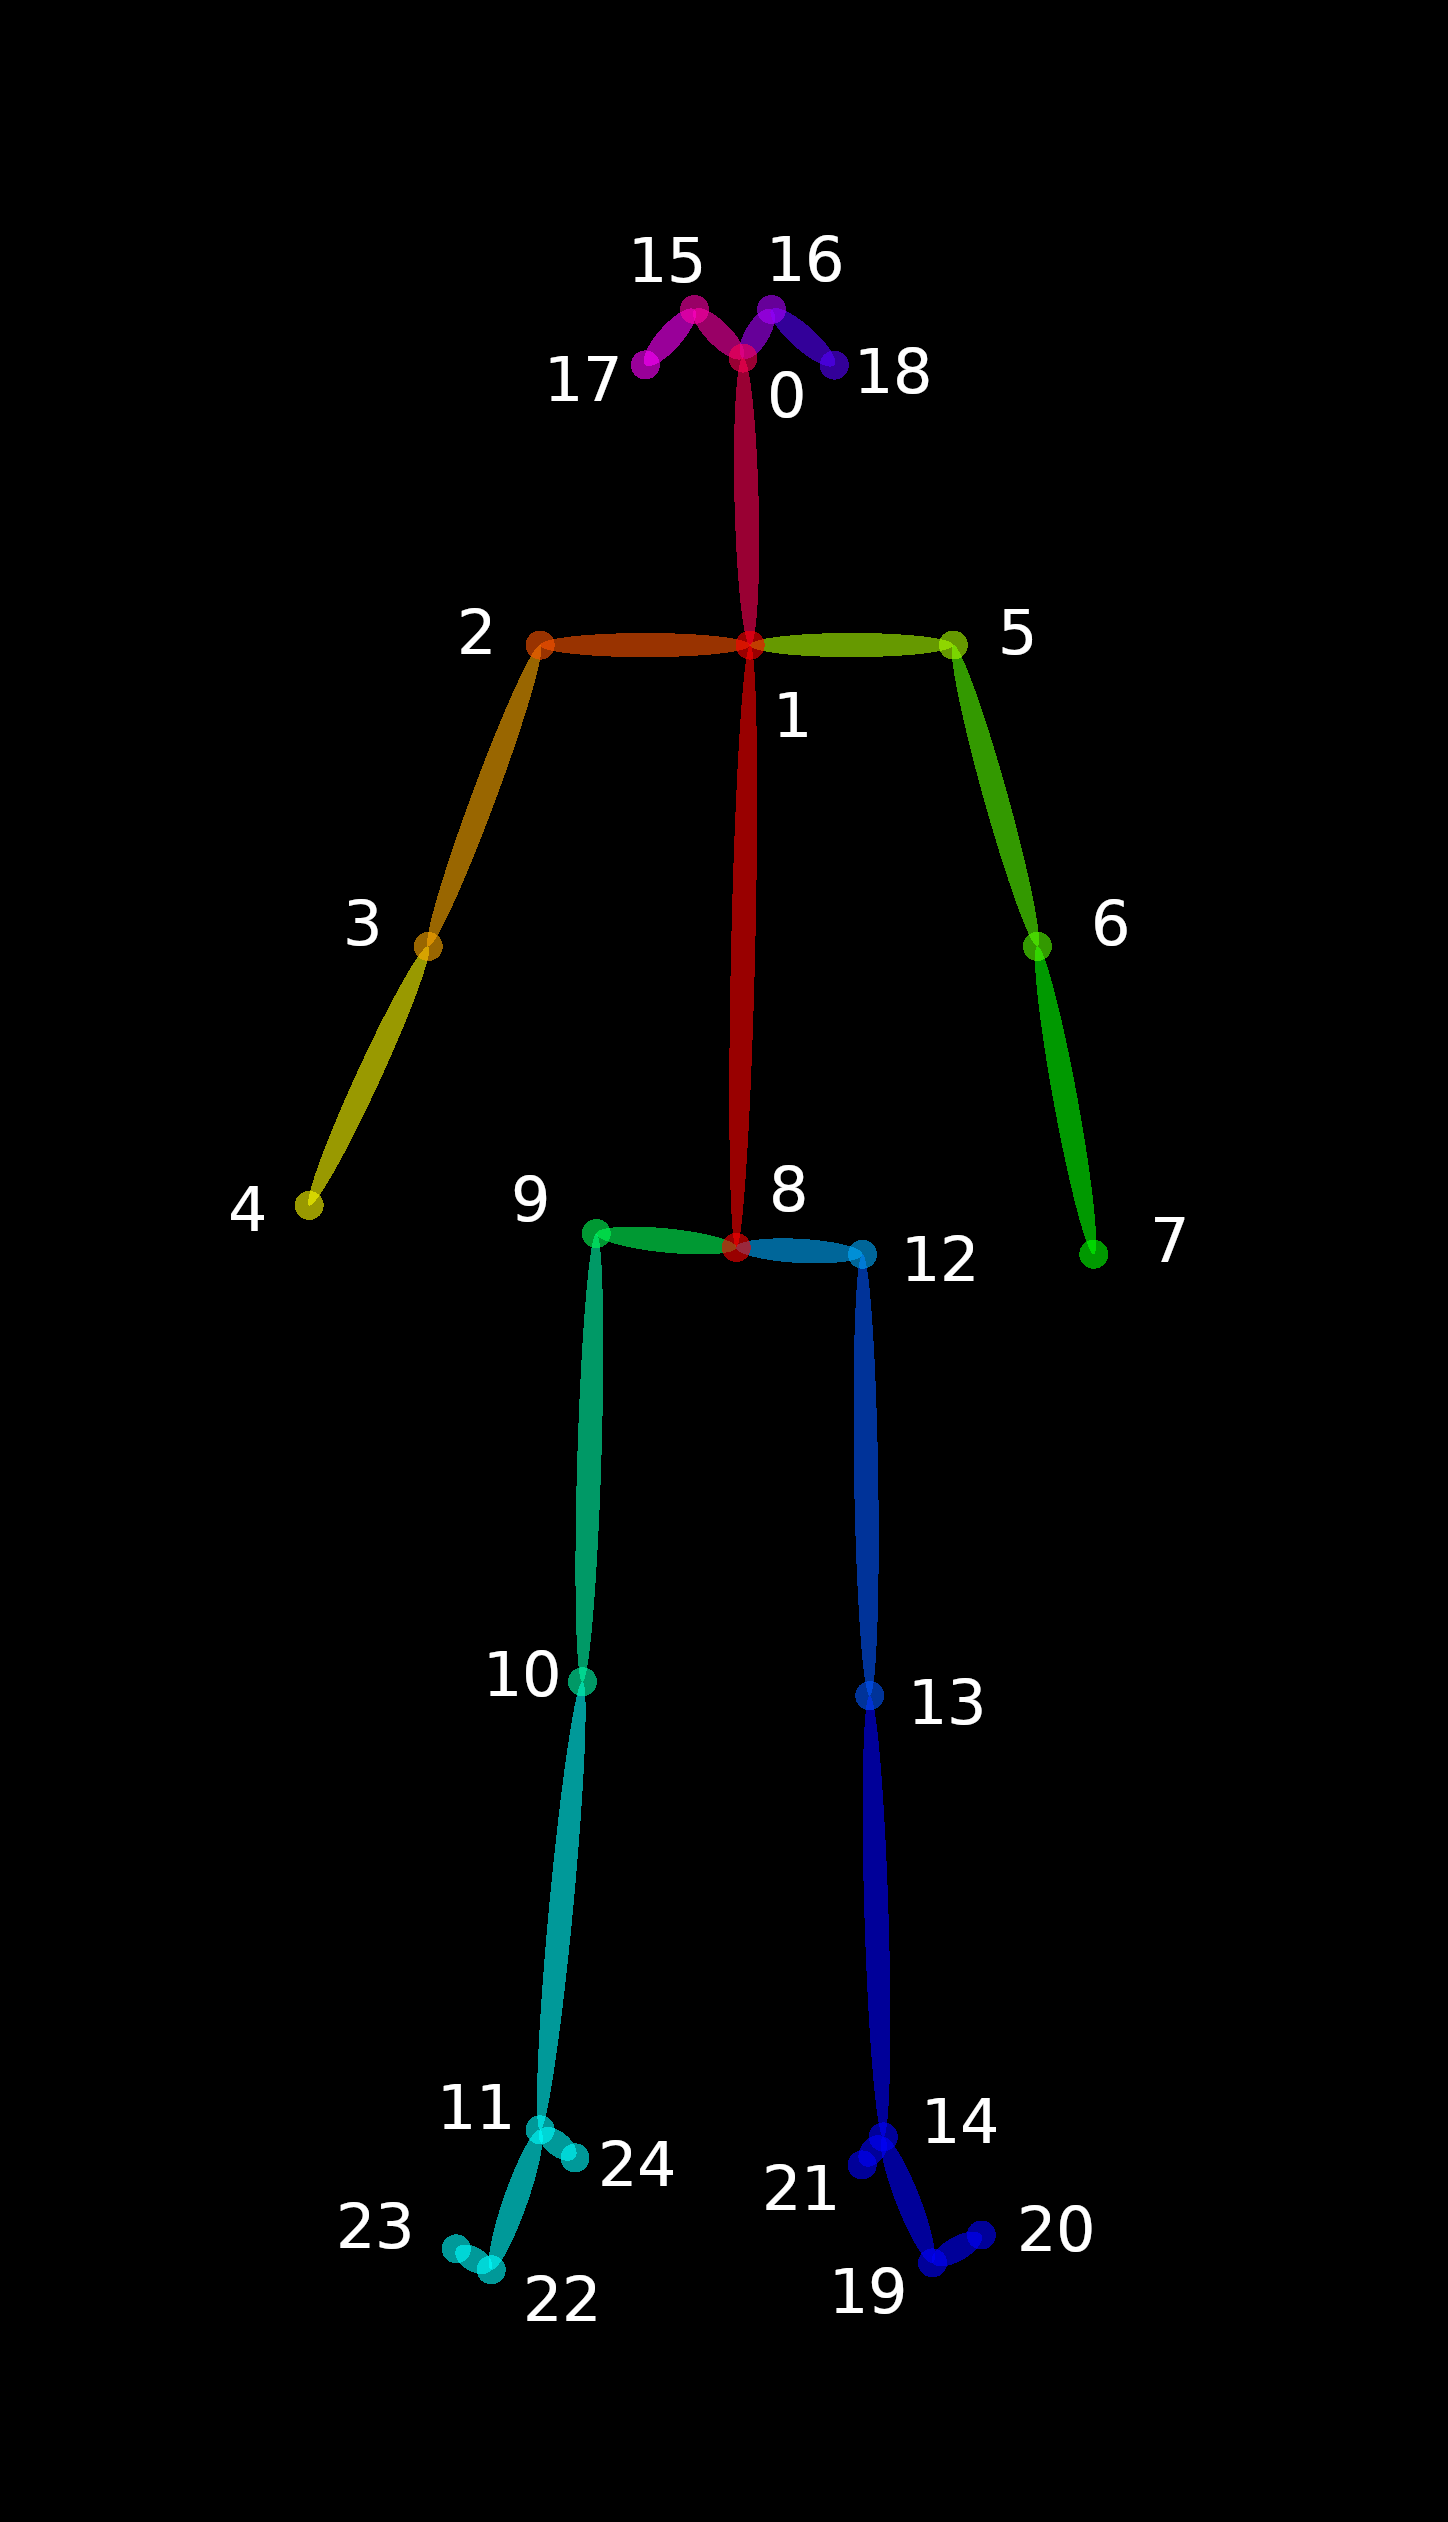
\includegraphics[width=0.2\linewidth]{img/chapter4_analysis/keypoints_pose_25.png}
	\caption{Keypoints produced by the BODY\_25 model \cite{Cao2017}.}
	\label{fig:bodyKeyPoints}
\end{figure}


\subsubsection{Head Pose Estimation}
We initially began the project by exploring the use of head-gaze estimation as a novel way of inferring the intended direction of motion of a person. We researched the concept of head pose estimation in Section \ref{sec:backHeadPoseEstimation}, with the logic being people tend to look in the direction where they are walking. We leveraged the use of the DeepGaze library as an initial starting point \cite{Patacchiola2017a}, since the library has a built in head-pose estimator. 

\begin{figure}[ht]
	\centering
	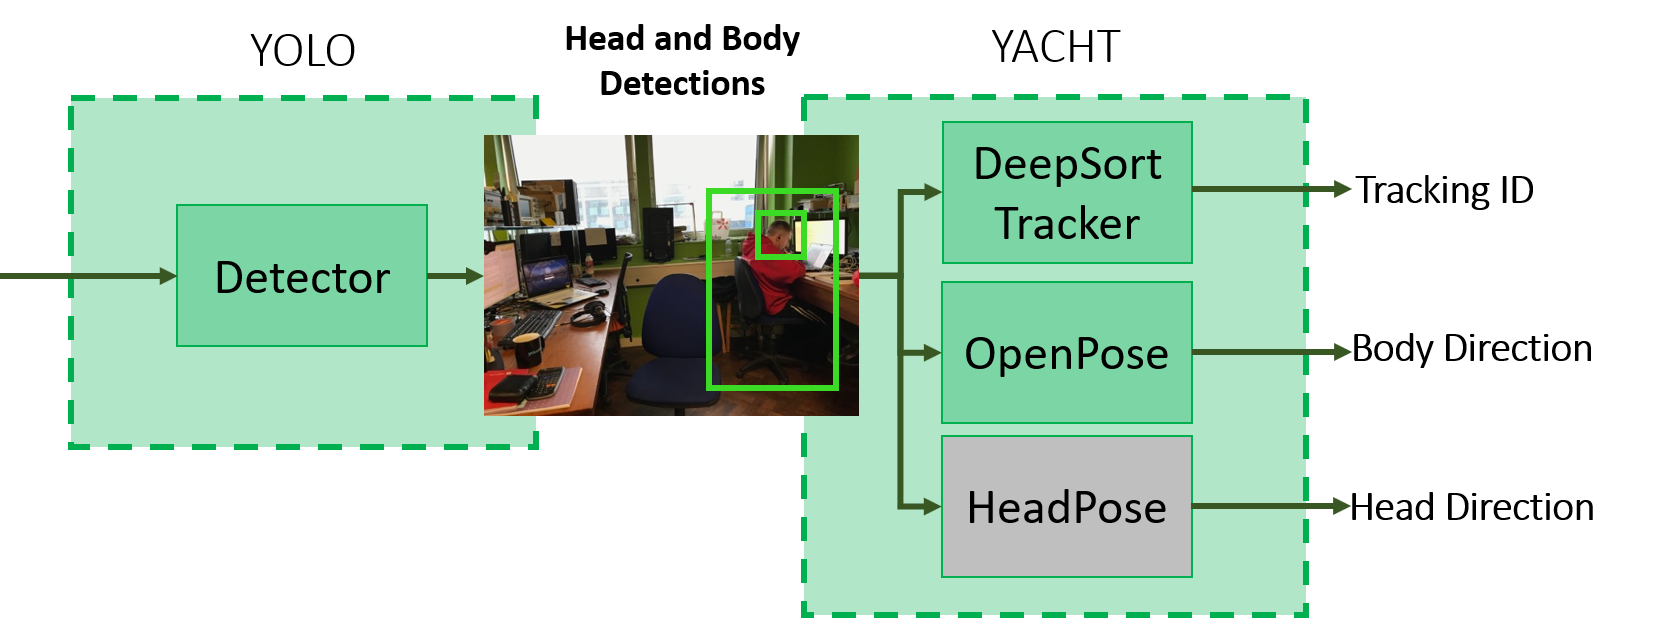
\includegraphics[width=1.0\linewidth]{img/chapter4_analysis/hddSystemHeadPose.png}
	\caption{Initial HDD System with the HeadPose Node before removal.}
	\label{fig:headPoseHDD}
	\vspace{-1\baselineskip}
\end{figure}

\paragraph{Head Detection} For this approach, we trained the YOLO detector to detect heads using the annotated CrowdHuman dataset. The head detections are consumed by the HeadPose node, which produces head pose projections that are sent to the Hololens.

\begin{figure}[ht]
	\begin{subfigure}[b]{.5\textwidth}
		\centering
		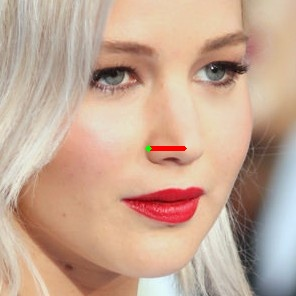
\includegraphics[width=0.675\linewidth]{img/chapter4_analysis/headPose.jpeg}
		\caption{Head pose estimation on close-up of face.}
	\end{subfigure}%
	\hspace{\fill} 
	\begin{subfigure}[b]{.5\textwidth}
		\centering
		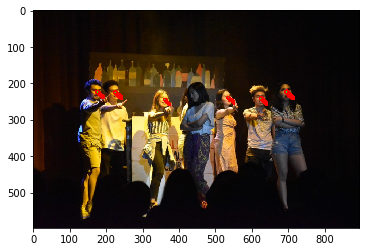
\includegraphics[width=1.0\linewidth]{img/chapter4_analysis/deepgazeWhole.png}
		\caption{Estimation on people at a distance.}
	\end{subfigure}
	\vspace{-2\baselineskip}
	\begin{center}
		\caption{DeepGaze head pose estimator on sample images. We notice in (b) that DeepGaze predicts everyone to be looking in the same direction, despite the differences in head poses.}
		\label{fig:deepGaze}
	\end{center}
	\vspace{-2\baselineskip}
\end{figure}

\paragraph{Reasons for removal} We noticed from our research that the head pose estimation was not very accurate, as can be seen in Figure \ref{fig:deepGaze}. A close up image of a face still returns an inaccurate estimation of the head pose. For smaller faces with multiple detections, the head pose estimation was not performed in real-time and also produced inaccurate estimations. Finally, as we will explain in the implementation section, the quality of the images received from the Hololens was too low, and as such, facial landmark detectors required for head pose estimation were unable to detect the key-points.

\section{Hololens Unity Application}
The Microsoft Hololens is a key component of this project since it acts as the main input, visualization and mapping device. To begin, we utilize the world-facing camera, which sees what the PWU is looking at as the input to the HDD system. Further along the processing pipeline, the Hololens Unity application receives the image co-ordinates of human detections and respective directions to build up a map of the objects in the surroundings. The application manages the holograms, keeping track of the world co-ordinates of the objects, which it sends to ARTA for the reactive control of the wheelchair.
This section covers how the system was designed so that it could be used in conjunction with other ROS nodes despite being a Unity application. It also describes the approach used to develop a front-camera stream, as well as a high level description of the modules responsible for the world mapping and hologram visualization.

\subsection{ROS Node} \label{sec:rossharp}
Both ARTA and the HDD are implemented on the Robotic Operating System as ROS nodes, and communicate with their sub-nodes using ROS messages across topics. As explained in Section \ref{sec:systemComms}, we view each of the three sub-systems as individual ROS nodes. However, the Hololens does not natively support ROS.

\begin{figure}[ht!]
	\centering
	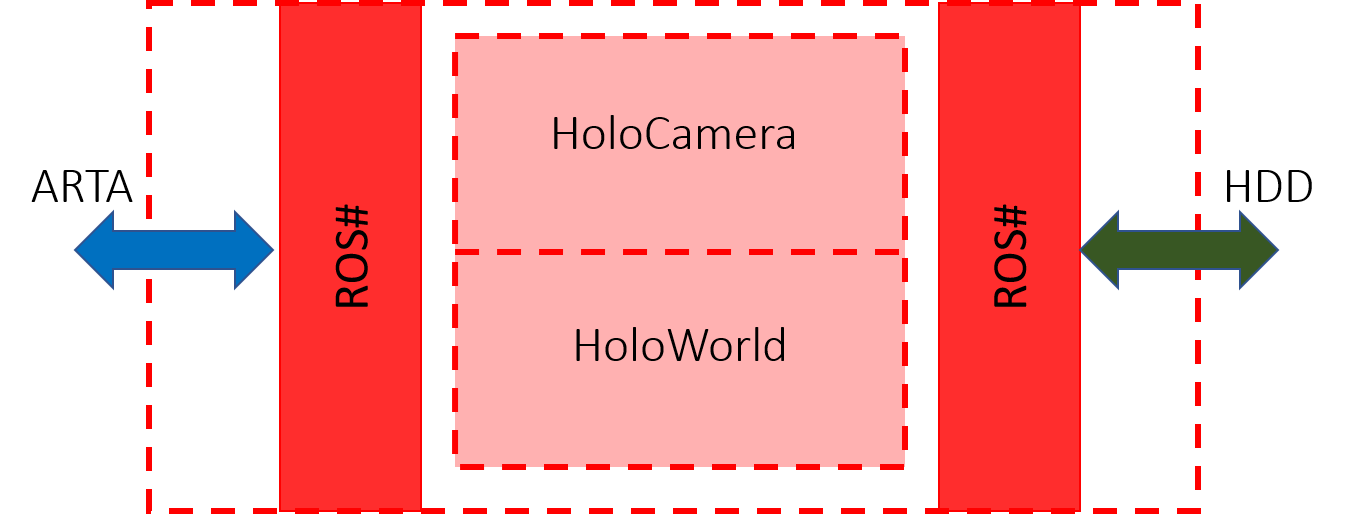
\includegraphics[width=0.8\linewidth]{img/chapter4_analysis/holoROSSharpWrapper.png}
	\caption{ROS\# acts as a ROS wrapper around the Unity application, allowing for seamless communication with other ROS nodes.}
	\label{fig:holoROSWrapper}
	\vspace{-1\baselineskip}
\end{figure}

\paragraph{} Since ROS is unable to be run on UWP, we had to use the \textbf{ROS\#} library implemented by Siemens. This allows Unity/UWP applications to send and receive data in the form of ROS messages across topics. Figure \ref{fig:holoROSWrapper} shows how the Unity application is viewed from other ROS nodes as just another node which it can communicate with using topics. The full implementation details of the ROS wrapping are covered later in this report. 

\subsection{HoloCamera}
We begin the Unity application analysis by starting at the beginning of the system pipeline. The HoloCamera is the main visual input to the whole system, prompting the need for a video camera stream to be developed. Previous work done in the PRL have used stationary images taken with the Hololens, but the process of streaming live video from the front camera is a new direction of development. Due to the importance of this step, we spent time researching methods of video streaming to an external computer.

\subsubsection{Video Streaming Choices} \label{sec:videoStreaming}

\paragraph{Windows Device Portal} Microsoft provides a portal to access the Hololens device configuration from a web browser. From the portal, we can manage the connection, control what applications are running and most importantly, access a video stream of the front-facing camera. However, after some testing, we realized that there is a delay of 1-2 seconds between the camera and the video rendered on the computer, making it unsuitable for this project.

\paragraph{Microsoft HoloLensForCV} Another option that was explored was the computer vision development tools released by Microsoft for the Hololens. This library provides developer access to the live camera stream, as well as the raw sensor data, such as the depth and IMU. This would have been the ideal video streaming choice. However, at the beginning of the project, we were not so experienced with developing UWP applications in C\#. Furthermore, it proved difficult to stream the sensor and video streams from a UWP device to a Linux machine, since Windows and Linux have different data formats and standards.

\paragraph{Unity Camera Stream} From our research, we found the \textbf{Vulcan Technologies Hololens Camera Stream} Unity add-on library. The community support for Unity development on the Hololens is immense, with various libraries such as the Mixed Reality Toolkit (MRTK) and many other Hololens specific tools. Furthermore, the 3D world modelling and spatial mapping capabilities available in Unity extend the capabilities of an augmented reality system. It abstracts away the complexities of the raw Hololens sensor data, reducing the time to market of applications. Finally, previous work in the PRL involving the Hololens have relied on Unity, making it an ideal choice for this project.

\subsubsection{Module Description}
The HoloCamera module is responsible for accessing the front-camera of the Hololens, compressing the raw image data into a JPEG format and streaming the video frames over the network. The application produces a ROS Compressed Image message that is sent to the HDD for object detection. We provide a complete explanation of the process in the implementation part of this report.

\subsection{HoloWorld}
The goal of this project was to develop an augmented reality system that will assist PWU in navigation by providing visual cues of people in the surroundings. Unity applications have the ability to place holograms in the users surroundings, and render them on the Hololens screen for the user to see. While the majority of the object detection and inference is done on an external computer, the Unity application on the Hololens is used to convert the image co-ordinates of objects into their 3D position in the world. Furthermore, the map of the surroundings is used by the reactive control component of ARTA to avoid collisions with the detected object, making the HoloWorld module a key component of the overall system.

\subsubsection{World Manager}
Since the Hololens is the intermediary, the World Manager sub-module is responsible for managing all the ROS topics between the Hololens, the HDD system and ARTA. The module receives the image co-ordinates from the HDD system and projects the detected points into the world frame. This returns a set of world co-ordinates which we can assign holographic visualizations and map in the Unity world surrounding the Hololens.

\subsubsection{ARTA Manager} \label{sec:alignment}
This module is a representation of ARTA in the Hololens world. It subscribes to topics published by ARTA that contain information about the robot, such as the position in the real world, the linear velocities and other published topics. 

\paragraph{Alignment}With most visual SLAM implementations, the camera attached to the mobile robot is fixed to the robots frame. This simplifies the conversion of the image co-ordinates to the robot frame, and then to the world frame. However, when a PWU wears the Hololens, the front-camera has the ability to move in 6 degrees of freedom. Most importantly, the PWU can turn their head to look left and right. This brings up the issue of not knowing whether a detected object is actually in front of the powered wheelchair, or if the PWU is looking at an object to the side. 

\begin{figure}[ht!]
	\centering
	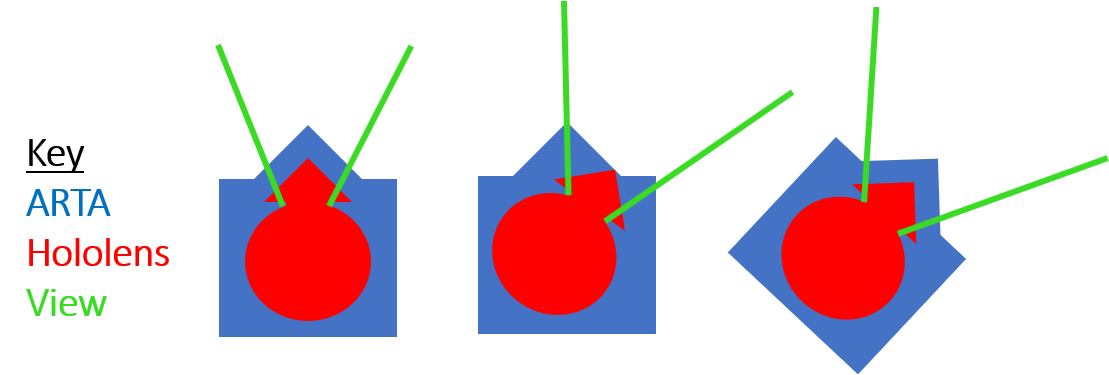
\includegraphics[width=0.9\linewidth]{img/chapter4_analysis/holoArtaAligned.png}
	\caption{We need a way of knowing if a detected object is in front of the wheelchair, or if the PWU is looking to the side. }
	\label{fig:holoArtaAlignment}
\end{figure}

\paragraph{}We visualize this problem in Figure \ref{fig:holoArtaAlignment}. When the Hololens camera and wheelchair frames are aligned, it is easy to tell if an object is in the path of the wheelchair. For the reactive control component of ARTA, we need to know if an object is in ARTAs current trajectory to determine if a collision will occur. As such, This module is responsible for discerning between people being in front of the wheelchair or to the side. 

\paragraph{Reactive Control} Furthermore, the ARTA Manager is responsible for consuming the navigation and localisation topics from the powered wheelchair and translating them to positions in the AR world of the Unity application. By modelling the wheelchair as an object in this world, the reactive control system can calculate the distance between the wheelchair and people detected in the surroundings. We can convert these distances and combine them with the manual input signals received from ARTA to avoid collisions with the detected individuals.

\section{ARTA}
The Personal Robotics Lab (PRL) at Imperial College London have built and developed an original smart powered wheelchair known as the Assistive Robotic Transport for Adults (ARTA). The wheelchair was designed to assist adults with mobility issues, and is frequently used in the PRL as a research topic in conjunction with exotic control interfaces such as the Hololens \cite{Zolotas2018, Chacon-Quesada}.

\subsection{ROS Packages}
Due to the previous work done on ARTA, the PRL have developed several ROS packages for the control of the powered wheelchair. These packages are used to combine data from the sensors attached to the wheelchair, using the data for localisation of the mobile robot and accepting manual input from the PWU in the form of joystick commands. We use these packages as a base system to build upon for our reactive control module.

\subsection{Reactive Control}
The powered wheelchair implements the physical part of the reactive control system project goals outlined in Section \ref{sec:reactive}. By understanding the PWU input control signals from the joystick of the wheelchair, a system was developed which uses the signals to determine if collisions with people in the surroundings will occur. The system also implements the reactive control aspect, which overrides the control signals sent by the PWU to avoid collisions.

\subsection{Removal of Exotic Control Interfaces}
In the interim report, we proposed the use of eye gaze tracking as a form of wheelchair control. We proposed the use of the Pupil Labs eye tracker add-on for the Hololens as a way of determining a point the user is looking at and moving the wheelchair autonomously there. We further proposed the use of the eye tracker to determine whether the PWU had noticed a person walking into the trajectory of the wheelchair. Fortunately, the members of the PRL have already implemented similar control interfaces for ARTA using the Hololens, and developed them in the \code{wheelchair\_control} ROS package.

\paragraph{}As the project progressed, we encountered an issue with image compression. Due to the limitations of the Unity engine, image compression of frames captured by the front facing camera can only be done on the main thread of the application. This thread is also responsible for displaying the augmented reality experience and rendering holograms. As such, the Unity application displays its content at 5 frames per second (FPS), well below the targeted 60 FPS level recommended by Pupil Labs for augmented reality experiences. We explain this issue in the implementation section of the report.

\paragraph{}Through experimentation, we found it was difficult to use the eye tracker plugin provided by Pupil Labs and maintain a video stream of the front facing camera simultaneously. Code profiling showed that the main thread spent more time compressing the raw images into JPEG format, and this did not give ample thread time for the eye tracker plugin to work properly. As such, we decided to remove the exotic control interface to focus on the reactive control aspect of the project.